% -------------------------------------------------------------------------------

% Génère deux pdf, avec et sans les overlays.

\ifdefined\ishandout
  \documentclass[handout]{beamer}
\else
  \documentclass{beamer}
\fi

% -------------------------------------------------------------------------------

% For sans serif fonts compiled with lualatex. Better for presentations.

%\fontspec[Scale=MatchLowercase]{Trebuchet MS}

% -------------------------------------------------------------------------------

% For regular serif fonts compiled with pdflatex

%\usepackage[T1]{fontenc} 
%\usepackage[utf8]{inputenc}

% -------------------------------------------------------------------------------

% Packages and settings

\usepackage[french,english]{babel}
\usepackage[utf8]{inputenc}
\usepackage[T1]{fontenc}

\usepackage{algorithm,algorithmic}
\usepackage{framed} % Put frames around text
\usepackage{textpos} % Put text on slides with (pos_x, pos_y)

\usepackage{mdframed}

\usepackage[binary-units,per-mode=symbol]{siunitx}
\usepackage{todonotes}
\usepackage{pgfplots}

\usepackage{caption}
\captionsetup[figure]{labelformat=empty}%

\graphicspath{{figures/}}
\pgfplotsset{
    compat=1.12,
    tick label style={font=\small},
    label style={font=\small},
    legend style={font=\small},
    /pgfplots/short line legend/.style={
        legend image code/.code={
            \draw[mark repeat=2,mark phase=2,##1]
            plot coordinates {
                (0cm,0cm)
                (0.2cm,0cm)
                (0.4cm,0cm)
            };%
        }
    },
    /pgfplots/xtick pos=left,
}

\usepgfplotslibrary{dateplot, groupplots, units, colorbrewer}

\setlength{\unitlength}{1cm}

% -------------------------------------------------------------------------------

% Generates a section frame with the title as an input argument
\newcommand{\sectionframe}[1]
{
\section[aaa]{#1}
\begin{frame}[plain]
\Large
  \begin{snugshade}
    \begin{center}
    \tc{#1}
  \end{center}
\end{snugshade}
\vspace{3cm}\mbox{}
\end{frame}
}

% -------------------------------------------------------------------------------

% Definitions

\newcommand{\pr}{\text{Pr}} % probabilities in math mode

\newcommand{\N}{\ensuremath{\mathbb{N}}\xspace}
\newcommand{\Z}{\ensuremath{\mathbb{Z}}\xspace}
\newcommand{\R}{\ensuremath{\mathbb{R}}\xspace}
\newcommand{\Q}{\ensuremath{\mathbb{Q}}\xspace}

\newcommand{\K}{\ensuremath{\mathcal{K}}\xspace}
\newcommand{\X}{\ensuremath{\mathcal{X}}\xspace}
\newcommand{\Y}{\ensuremath{\mathcal{Y}}\xspace}

% Logical operators
\renewcommand{\lnot}{\neg}
\newcommand{\lxor}{\oplus}
\newcommand{\lif}{\rightarrow}
\newcommand{\liff}{\leftrightarrow}
\newcommand{\lnand}{\mid}
\newcommand{\lnor}{\downarrow}

\newcommand{\tc}[1]{{\color{tc}#1}} % Theme color for the text

% Parametrized names for the system
\newcommand{\epto}{\textsc{EpTO}\xspace}
\newcommand{\jgroups}{\textsc{JGroups}\xspace}
\newcommand{\sys}{\textsc{EpTOTester}\xspace}

% -------------------------------------------------------------------------------

% Colors

\newcommand{\colorformatblue}
{
\definecolor{tc}{rgb}{0.2,0,0.4}
\colorlet{backcolor}{tc!15!white}
\colorlet{shadecolor}{tc!10!white}
}

\newcommand{\colorformatgreen}
{
\definecolor{tc}{rgb}{0,0.3,0}
\colorlet{backcolor}{tc!30!white}
\colorlet{shadecolor}{tc!30!white}
}

\newcommand{\colorformatred}
{
\definecolor{tc}{rgb}{0.5,0,0}
\colorlet{backcolor}{tc!30!white}
\colorlet{shadecolor}{tc!10!white}
}

\newcommand{\colorformatpurple}
{
\definecolor{tc}{rgb}{0.5,0,0.5}
\colorlet{backcolor}{tc!30!white}
\colorlet{shadecolor}{tc!10!white}
}

\newcommand{\colorformatgray}
{
\definecolor{tc}{rgb}{0.5,0.5,0.5}
\colorlet{backcolor}{tc!40!white}
\colorlet{shadecolor}{tc!40!white}
}

\newcommand{\colorformatpink}
{
\definecolor{tc}{rgb}{0.8,0.2,0.8}
\colorlet{backcolor}{tc!40!white}
\colorlet{shadecolor}{tc!40!white}
}

\newcommand{\colorformatorange}
{
\definecolor{tc}{rgb}{1,0.7,0.4}
\colorlet{backcolor}{tc!40!white}
\colorlet{shadecolor}{tc!40!white}
}

\newcommand{\colorformatcornflowerblue}
{
\definecolor{tc}{rgb}{0.39,0.58,0.93}
\colorlet{backcolor}{tc!40!white}
\colorlet{shadecolor}{tc!40!white}
}

% -------------------------------------------------------------------------------

\usetheme{metropolis}

% To include a logo in each slide
% \logo{
\includegraphics[width=1cm\vspace{-1cm}]{unine}}

\setbeamertemplate{navigation symbols}{}

\title[\sys]{\textbf{EpTOTester: \\ Implementation of Large-Scale\\ Epidemic Total Order Algorithms}}

\author[]{\textbf{Jocelyn Thode}, Hugues Mercier, Miguel Matos}

\subtitle[]{Master Thesis}

\institute[]{Department of Informatics \\ University of Fribourg, Switzerland \\  \href{mailto:jocelyn.thode@unifr.ch}{jocelyn.thode@unifr.ch}} 
\date[\today]{Neuchâtel, Switzerland, \today}

\setbeamertemplate{frame footer}{%
	\parbox{\linewidth}{Master Thesis \hfill \insertshorttitle\ \ - \  \insertshortsubtitle \hfill \href{mailto:jocelyn.thode@unifr.ch}{jocelyn.thode@unifr.ch}}} 
%\setbeamertemplate{footline}[text line]{%
%\parbox{\linewidth}{\vspace*{-8pt}  Master Thesis \hfill \insertshorttitle\ \ - \  \insertshortsubtitle \hfill \href{mailto:jocelyn.thode@unifr.ch}{jocelyn.thode@unifr.ch} \hfill \hfill\insertframenumber}} 

\setbeamertemplate{navigation symbols}{}

% Beamer footline without logo
%\setbeamertemplate{footline}[text line]{%
%\vspace*{-8pt} \insertsh \ - \insertshortsubtitle \hfill \insertframenumber \hspace{-0.5cm}}

% This allows to set pdf bookmarks at the frame level
%\usepackage{bookmark}
%\makeatletter
%\apptocmd{\beamer@@frametitle}{\only<1>{\bookmark[page=\the\c@page,level=3]{#1}}}
%\makeatother

% -------------------------------------------------------------------------------

\setbeamercovered{transparent}

\begin{document}

% -------------------------------------------------------------------------------
% -------------------------------------------------------------------------------

\begin{frame}[plain]
  
\titlepage

\end{frame}

% -------------------------------------------------------------------------------
% -------------------------------------------------------------------------------

\subtitle[Outline]{Outline}

\begin{frame}{Outline}
    \begin{itemize}
        \item Motivation
        \item \epto{} explained
        \item \sys
        \item Evaluation
        \item Conclusion
    \end{itemize}
\end{frame}

\section{Introduction}
\subtitle[Introduction]{Introduction}

\begin{frame}{Motivation}
    \epto{} was only evaluated using a \textbf{simulation}. We need an evaluation with real peers to:
    \begin{itemize}
    	\item Expose possible \textbf{limitations}
    	\item Confirm simulation \textbf{results}
    \end{itemize} 
\end{frame}

\begin{frame}{Motivation}
  \begin{itemize}
  \item Comparing \epto{} meant testing it against other algorithms
  \item No framework to easily benchmark algorithms without having to rewrite them
  \end{itemize}

\end{frame}

\subtitle[Description]{Description}

\begin{frame}{What is \epto{}?}
	\textbf{Epidemic Total Order Algorithm:}
	\begin{itemize}
		\item Probabilistic dissemination algorithm
			\begin{itemize}
				\item Using balls-and-bins
			\end{itemize}
		\item Provides deterministic total order
		\item Scales in the number of peers and events
			\begin{itemize}
				\item Parameters increase logarithmically
			\end{itemize}
		\item Churn resistant
	\end{itemize}
\end{frame}

%\begin{frame}{What is \epto{}? (2)}
%	\textbf{Properties satisfied:}
%\begin{itemize}
%	\item Integrity
%	\item Validity
%	\item Total Order
%	\item Probabilistic Agreement
%\end{itemize}
%\end{frame}

%\begin{frame}{Properties satisfied}
%	\begin{itemize}
%		\item Integrity
%		\item Validity
%		\item Total Order
%		\item Probabilistic Agreement
%	\end{itemize}
%\end{frame}
\begin{frame}{\epto{} architecture}
    \begin{figure}
        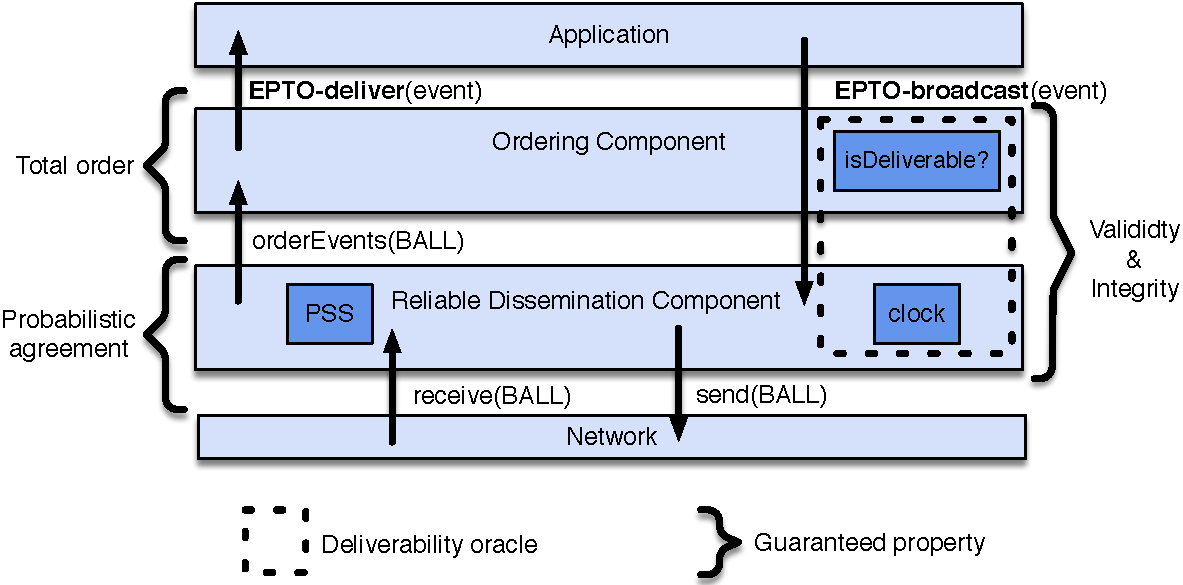
\includegraphics[scale=0.5]{figures/architecture}
    \end{figure}
\tiny{M. Matos, H. Mercier, P. Felber, R. Oliveira and J. Pereira, “EpTO: An epidemic total order algorithm for Large-scale distributed systems”, in Proceedings of the 16th Annual Middleware Conference, ACM, 2015, pp. 100–111.
}
\end{frame}

\begin{frame}{\sys{} features}
    \begin{itemize}
    	\item Compatible with any distributed algorithm provided it runs on Docker
    	\item support for a user-provided tracker
    	\item Automated benchmarking execution
    	\item Containers allow for more than 1 peer per physical node
    	\item Can simulate churn or follow real traces
    \end{itemize}
\end{frame}

\begin{frame}{\sys{} architecture}
	\begin{figure}
		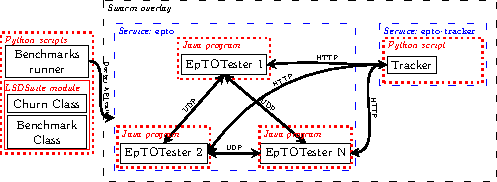
\includegraphics[scale=1.2]{complete-architecture}
	\end{figure}
\end{frame}

\begin{frame}{\sys{} Configuration and Logging}
	The protocol, churn and framework configuration is done through \textsc{YAML} files
	
	The protocols logs must be written in a file to be extracted to the host
\end{frame}

\section{Evaluation}
\subtitle[Evaluation]{Evaluation}

\begin{frame}{Evaluation}
    We evaluate \epto{} against \jgroups{} according scaling peers and global event throughput per second.
    
    We write $(n,e)$ where $n$ is the number of peers and $e$ is the global event throughput per second.
\end{frame}

\begin{frame}{Bandwidth}
	\begin{figure}
		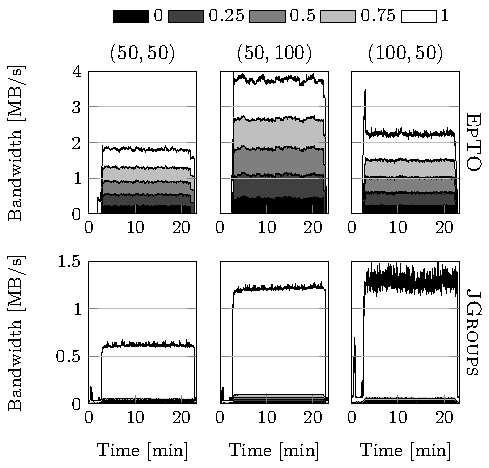
\includegraphics[scale=0.9]{bandwidth-nochurn}
	\end{figure}
\end{frame}

\begin{frame}{Bandwidth Synthetic Churn $(100,50)$}
	\begin{figure}
		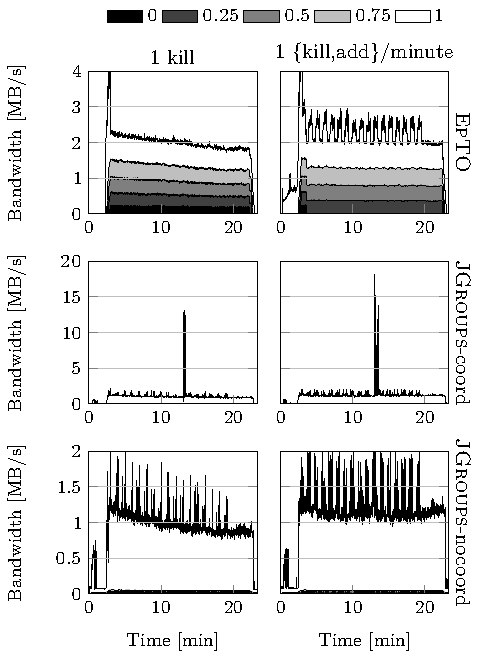
\includegraphics[scale=0.68]{bandwidth-synth-churn}
	\end{figure}
\end{frame}

\begin{frame}{Bandwidth Real Churn}
	\begin{figure}
		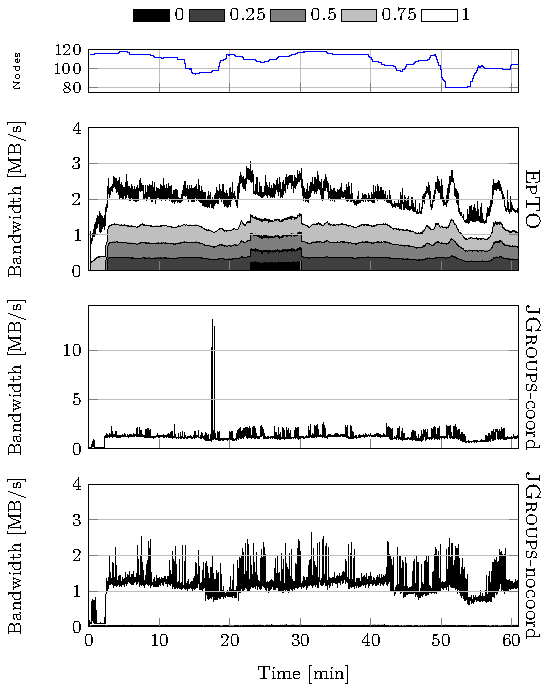
\includegraphics[scale=0.65]{bandwidth-real-churn}
	\end{figure}
\end{frame}

\begin{frame}{Local Dissemination Stretch}
	\begin{figure}
		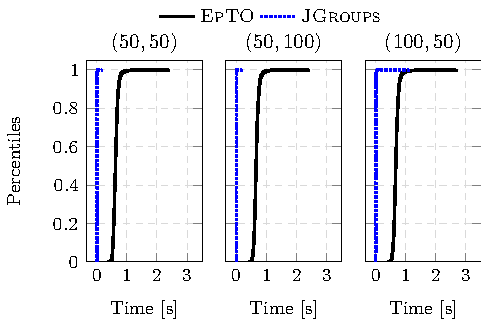
\includegraphics[scale=1]{local-diss-stretch-nochurn}
	\end{figure}
\end{frame}

\begin{frame}{Local Dissemination Stretch Synthetic Churn $(100,50)$}
	\begin{figure}
		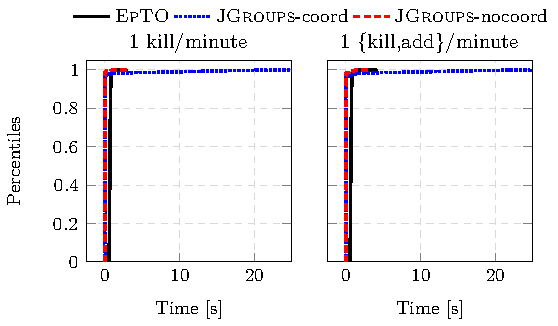
\includegraphics[scale=1]{local-diss-stretch-synth-churn}
	\end{figure}
\end{frame}

\begin{frame}{Local Dissemination Stretch Real Churn}
	\begin{figure}
		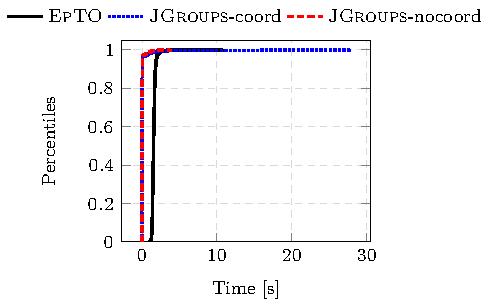
\includegraphics[scale=1]{local-diss-stretch-real-churn}
	\end{figure}
\end{frame}

\begin{frame}{Local Times}
	\begin{figure}
		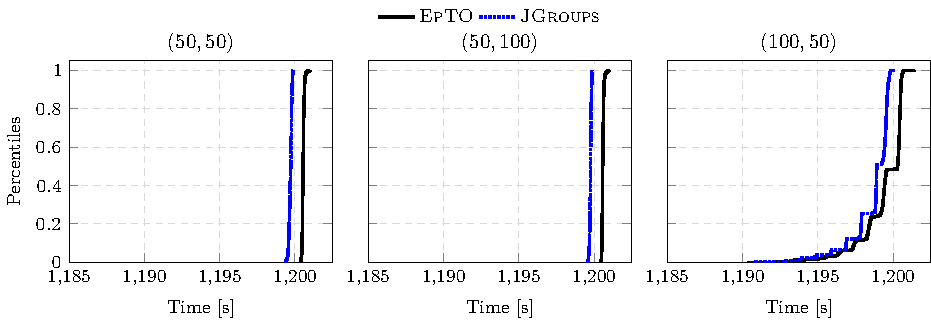
\includegraphics[scale=0.70]{local-times-nochurn}
	\end{figure}
\end{frame}

\begin{frame}{Local Times Synthetic Churn $(100,50)$}
	\begin{figure}
		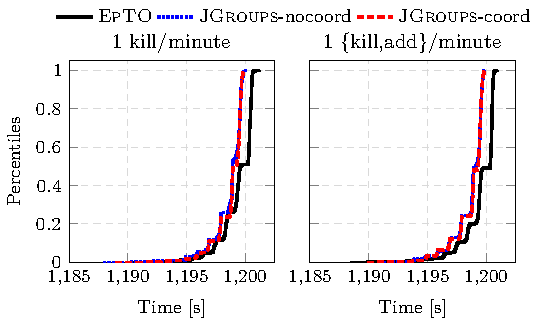
\includegraphics[scale=1]{local-times-synth-churn}
	\end{figure}
\end{frame}

\begin{frame}{Local Times Real Churn}
	\begin{figure}
		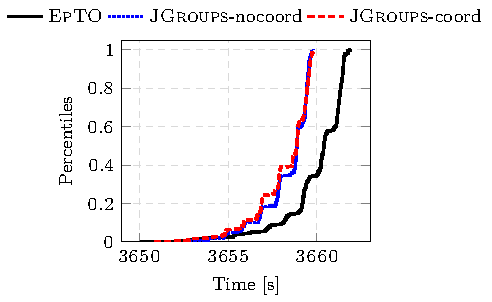
\includegraphics[scale=1]{local-times-real-churn}
	\end{figure}
\end{frame}

\begin{frame}{Total \si{\giga\byte} sent/received}
\begin{table}
	\sisetup{table-format=2.2, separate-uncertainty, table-figures-uncertainty = 2, table-align-uncertainty}
	\begin{tabular}{llSSS}
		\toprule
		&& \multicolumn{3}{c}{Cluster parameters} \\
		\cmidrule{3-5}
		{Protocol}&& {$(50,50)$} & {$(50,100)$} & {$(100,50)$} \\
		\midrule
		\multirow{2}{*}{\epto}&{Receive}& 10.84(016) & 22.31(039) & 26.01(027) \\
		&{Sending}& 10.84(016) & 22.31(039) & 26.01(027)\\
		\midrule
		\multirow{2}{*}{\jgroups}&{Receive}& 0.78(003) & 1.45(001) & 1.88(001)\\
		&{Sending}& 0.77(003) & 1.44(001) & 1.84(001)\\
		\bottomrule
	\end{tabular}
\end{table}
\end{frame}

\begin{frame}{Total events sent in a stable environment}
	\begin{table}
		\centering
		\sisetup{table-format=6.1, separate-uncertainty, table-figures-uncertainty = 2, table-align-uncertainty}
		\begin{tabular}{lSSS}
			\toprule
			& \multicolumn{3}{c}{Cluster parameters} \\
			\cmidrule{2-4}
			Protocol & {$(50,50)$} & {$(50,100)$} & {$(100,50)$} \\
			\midrule
			\epto & 59993.8(33) & 119898.2(97) & 59913.0(1643) \\
			\jgroups & 59961.9(109) & 119885.7(50) & 60023.1(2871) \\
			\bottomrule
		\end{tabular}
	\end{table}
\end{frame}

\begin{frame}{Total events sent with a synthetic churn $(100,50)$}
	\begin{table}
		\centering
		\sisetup{table-format=6.1, separate-uncertainty, table-figures-uncertainty = 2, table-align-uncertainty}
		\begin{tabular}{lSSS}
			\toprule
			& \multicolumn{2}{c}{Cluster parameters} \\
			\cmidrule{2-3}
			Protocol & {1 kill/minute} & {1\{kill,add\}/minute} \\
			\midrule
			\epto & 53898.5(1339) & 59798.6(1401) \\
			\jgroups-coord & 53834.7(1755) & 59507.9(2409) \\
			\jgroups-nocoord & 53830.5(2003) & 59450.5(1751) \\
			\bottomrule
		\end{tabular}
	\end{table}
\end{frame}

\begin{frame}{Total events sent during a real trace}
	\begin{table}
		\centering
		\sisetup{table-format=6.1, separate-uncertainty, table-figures-uncertainty = 6, table-align-uncertainty}
		\begin{tabular}{lS}
			\toprule
			Protocol & {Events sent}\\
			\midrule
			\epto & 165844.2(2102)\\
			\jgroups-coord & 166183.0(13681)\\
			\jgroups-nocoord & 166585.8(8249)\\
			\bottomrule
		\end{tabular}
	\end{table}
\end{frame}

\section{Conclusion}
\subtitle[Conclusion]{Conclusion}

\begin{frame}{Limitations}
	\begin{itemize}
		\item Difference not strong enough at 100 peers scale
		\item High CPU usage
		\item Docker problems on AWS/GCE
	\end{itemize}
\end{frame}

\begin{frame}{Future Work}
    \begin{itemize}
        \item Obtain more resources to have stronger results
        \item Implement a Push-Pull \epto{} version
        \item Use Kubernetes instead of Docker + Docker swarm
        \item Refine Framework Architecture
    \end{itemize}
\end{frame}

\begin{frame}[standout]
	Questions?
\end{frame}

\appendix

\begin{frame}{Total \si{\giga\byte} sent/received Synthetic Churn $(100,50)$}
	\begin{table}
		\centering
		\sisetup{table-format=2.2, separate-uncertainty, table-figures-uncertainty = 2, table-align-uncertainty}
		\begin{tabular}{lSSS}
			\toprule
			&& \multicolumn{2}{c}{Churn parameters} \\
			\cmidrule{3-4}
			{Protocol}&& {1 kill/minute} & {1\{kill,add\}/minute} \\
			\midrule
			\multirow{2}{*}{\epto}&{Receive}& 21.00(024) & 26.32(032)\\
			&{Sending}& 21.21(025) & 26.57(032)\\
			\midrule
			\multirow{2}{*}{\jgroups-coord}&{Receive}& 1.47(002) & 1.75(002)\\&{Sending}& 1.43(002) & 1.70(002)\\
			\midrule
			\multirow{2}{*}{\jgroups-nocoord}&{Receive}& 1.45(001) & 1.73(002)\\&{Sending}& 1.41(001) & 1.68(002)\\
			\bottomrule
		\end{tabular}
	\end{table}
\end{frame}

\begin{frame}{Total \si{\giga\byte} sent/received Real Churn}
	\begin{table}[hpt]
		\centering
		\sisetup{table-format=2.2, separate-uncertainty, table-figures-uncertainty = 2, table-align-uncertainty}
		\begin{tabular}{lSS}
			\toprule
			&& \multicolumn{1}{c}{Churn parameters} \\
			\cmidrule{3-3}
			{Protocol}&& {Real Trace} \\
			\midrule
			\multirow{2}{*}{\epto}&{Receive}& 81.41(108)\\
			&{Sending}& 82.67(108)\\
			\midrule
			\multirow{2}{*}{\jgroups-coord}&{Receive}& 5.56(008)\\
			&{Sending}& 5.40(008)\\
			\midrule
			\multirow{2}{*}{\jgroups-nocoord}&{Receive}& 5.58(005)\\
			&{Sending}& 5.43(005)\\
			\bottomrule
		\end{tabular}
	\end{table}
\end{frame}

\begin{frame}{Global Times}
	\begin{figure}
		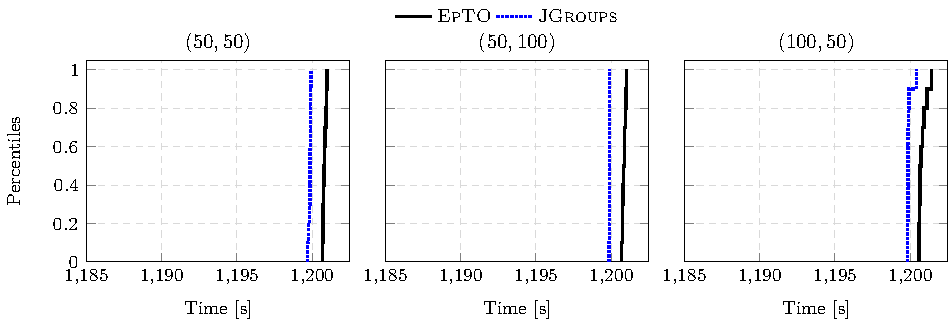
\includegraphics[scale=0.65]{global-times-nochurn}
	\end{figure}
\end{frame}

\begin{frame}{Global Times Synthetic Churn}
	\begin{figure}
		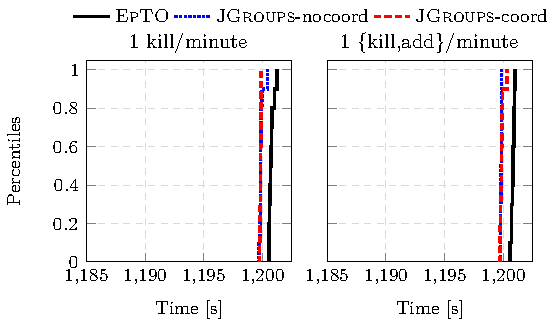
\includegraphics[scale=1]{global-times-synth-churn}
	\end{figure}
\end{frame}

\begin{frame}{Global Times Real Churn}
	\begin{figure}
		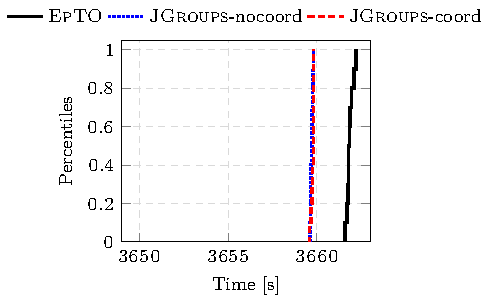
\includegraphics[scale=1]{global-times-real-churn}
	\end{figure}
\end{frame}

% -------------------------------------------------------------------------------
% -------------------------------------------------------------------------------

\end{document}

% -------------------------------------------------------------------------------

